\documentclass[10pt,a4paper]{article}

\usepackage[a4paper,margin=0.8in]{geometry}
\usepackage{xeCJK}
\usepackage{booktabs}
\usepackage{amsmath,amssymb}
\usepackage{array}
\usepackage{graphicx}
\usepackage{caption}
\usepackage{enumitem}
\usepackage{float}
\usepackage[colorlinks=true, linkcolor=blue, urlcolor=blue, citecolor=blue]{hyperref}

\title{Fantasy Baseball Draft Optimization \\[0.5em] \large OR114-2 Final Project, Group 4}
\author{
B13705051 周孟承 \and
B13902103 鄭宇宏 \and
B13303153 詹舒宇 \and
B11705039 李盈盈
}
\date{}

\begin{document}
\maketitle

\section{Introduction}

Fantasy baseball drafts require managers to build a competitive roster before the season even begins. In a snake draft, each manager owns only a fixed sequence of picks, while the available player pool is continually reshaped by opponents' selections and by market expectations summarized through average draft position (ADP). The practical decision is therefore not simply which players are strongest in isolation, but which players should be selected now before positional needs and market timing make better options disappear.

This decision is challenging because draft value is interdependent. A high-projection player may not be the best choice if he occupies an already abundant position, while a slightly lower-projection player may be more valuable if he protects a scarce roster slot. In practice, fantasy managers often rely on rankings, best-player-available rules, or manual judgment, but these shortcuts do not explicitly account for how one pick changes the value of the remaining roster. The decision maker must repeatedly balance projected points, positional scarcity, future availability, and computation time in a highly constrained environment.

We study this problem as an operations research decision-support task. An ADP-aware integer linear program provides an exact benchmark for smaller instances, while Direct Greedy serves as a simple baseline. Our proposed method, \emph{Opportunity Cost Greedy}, estimates the cost of waiting by comparing the current value of available players with the value likely to remain at the next owned pick. The goal is to preserve the strategic logic of the exact model while remaining fast enough for larger draft settings.

The report evaluates these methods on controlled synthetic instances and on real fantasy baseball data. The main message is a scalability trade-off: exact optimization gives a strong benchmark but becomes expensive as draft instances grow, whereas Opportunity Cost Greedy remains practical and consistently improves on the direct greedy baseline.

\section{Problem Description}

We consider a fantasy baseball snake draft in which a manager owns a fixed set of picks determined by draft order and the number of teams. At each owned pick, the manager must choose one available player from the remaining pool. Each player has a projected fantasy value, one or more eligible roster positions, and an ADP estimate that reflects when that player is expected to be drafted in the market.

The manager's goal is to construct a final roster that satisfies all positional requirements while maximizing total projected points. A player can only be drafted if he is still available at the current pick, and a drafted player can only be assigned to an eligible roster slot. The roster is not just a list of best individual names; it is a feasible lineup structure that must include the required number of catchers, infielders, outfielders, and pitchers.

The base roster used in the experiments has 16 slots. The utility slot is hitter-only, so pitchers cannot be assigned to \texttt{Util}. The same roster rules are used by the ILP, Direct Greedy, and Opportunity Cost Greedy, which keeps the comparison fair.

\begin{table}[H]
\centering
\small
\caption{Base fantasy baseball roster requirements.}
\label{tab:roster}
\begin{tabular}{lrrrrrrrrr}
\toprule
Position & C & 1B & 2B & 3B & SS & OF & Util & SP & RP \\
\midrule
Slots & 1 & 1 & 1 & 1 & 1 & 3 & 1 & 5 & 2 \\
\bottomrule
\end{tabular}
\end{table}

This problem is sequential in appearance but integrated in structure. A choice made early in the draft affects what remains possible later, especially when a position is scarce or when a player's market value suggests he may disappear before the manager's next turn. The core trade-off is between immediate value and future flexibility: taking the best current player may ignore the opportunity cost of leaving a critical position unresolved, while drafting for scarcity too early may sacrifice points if better overall value is still available.

From a business perspective, the question is a planning problem under uncertainty. The manager must choose among alternatives in a dynamic environment where opponents also act, player availability changes after every pick, and roster feasibility matters as much as raw player quality. This is why the project treats fantasy draft planning as an optimization and decision-support problem rather than a pure ranking exercise.

\section{Model Formulation}

Let $I$ be the set of players, $P$ the set of roster positions, and $K$ the set of owned draft picks. Each player $i \in I$ has projected points $v_i$, ADP $\text{adp}_i$, and a set of eligible positions $E_i \subseteq P$. Each roster position $p \in P$ has a required count $r_p$. The draft order determines the pick number associated with each owned pick $k \in K$.

We use the following decision variables:
\begin{itemize}[leftmargin=1.5em]
  \item $y_i \in \{0,1\}$, equal to 1 if player $i$ is drafted;
  \item $x_{ip} \in \{0,1\}$, equal to 1 if player $i$ is assigned to position $p$;
  \item $z_{ik} \in \{0,1\}$, equal to 1 if player $i$ is selected with owned pick $k$.
\end{itemize}

The objective is to maximize total projected roster points:
\[
\max \sum_{i \in I} v_i y_i.
\]

The model includes the following constraints. First, each owned pick must select exactly one player:
\[
\sum_{i \in I} z_{ik} = 1, \quad \forall k \in K.
\]
Second, each player can be selected at most once across all picks:
\[
\sum_{k \in K} z_{ik} \le 1, \quad \forall i \in I.
\]
Third, drafting a player must imply that he is assigned to exactly one roster position:
\[
\sum_{p \in P} x_{ip} = y_i, \quad \forall i \in I.
\]
Fourth, each drafted player may only be assigned to an eligible position:
\[
x_{ip} = 0 \quad \text{if } p \notin E_i.
\]
Fifth, each roster position must be filled exactly to its requirement:
\[
\sum_{i \in I} x_{ip} = r_p, \quad \forall p \in P.
\]

To enforce draft availability, we use an ADP-based restriction that prevents a player from being chosen if the current pick occurs too late relative to his expected market position. In the implementation, the ADP buffer parameter controls how strict this rule is. The exact form can be written as a feasibility condition on $z_{ik}$ based on the pick number of $k$ and the player's ADP. Binary restrictions apply to all decision variables.

Two modeling assumptions are worth stating explicitly. First, we treat projected points as the primary value signal, so the objective focuses on maximizing expected total fantasy production rather than category balance or bench construction. Second, we treat ADP as a market-availability proxy rather than a perfect predictor of human behavior. That is appropriate for this project because the goal is to build a practical draft tool, not to forecast every opponent's move exactly.

This formulation explains why an exact benchmark is valuable but not sufficient. It captures the integrated draft-planning problem precisely, while the live decision environment still motivates a faster heuristic.

\section{Algorithms}

This project compares one exact benchmark with two heuristic methods.

\subsection{ADP-aware ILP}

The ADP-aware integer linear program is the exact benchmark. It is solved with Gurobi and uses the full set of roster, eligibility, and availability constraints. When the instance is small enough, the ILP provides the best objective value and therefore serves as the reference for optimality-gap calculations.

Its strength is solution quality. Its weakness is scalability. As the player pool and roster structure grow, the number of binary variables and constraints increases quickly, and solve time can become large enough to limit practical use during drafting.

Conceptually, the ILP plays the role of a planning oracle. It is not meant to be used as a live drafting rule for every instance, but it provides the benchmark against which the heuristic methods are evaluated. This is especially important because the draft problem is not only about finding a feasible roster; it is about understanding how much value is lost when the algorithm must move from exact optimization to a faster approximation.

\subsection{Direct Greedy}

Direct Greedy is the simplest baseline heuristic. It makes decisions using only the current draft state and does not explicitly reason about the opportunity cost of waiting. In effect, it looks for a feasible player that fits an open roster need and has strong current value, then repeats the process until the roster is complete.

This method is fast and easy to interpret, which makes it a useful baseline. However, it is also myopic: if the algorithm fills a position too early or ignores a scarce role, it may later be forced into weaker choices.

Direct Greedy is intentionally simple. That makes it a clean comparison point: if Opportunity Cost Greedy cannot improve on such a straightforward baseline, then the proposed idea would not be meaningful. In practice, the baseline helps isolate whether the improvement comes from the opportunity-cost logic rather than from unrelated implementation tricks.

\subsection{Opportunity Cost Greedy}

Opportunity Cost Greedy is the project's proposed heuristic. The main idea is to evaluate not only the current value of taking a player now, but also the value that may be lost if the manager waits until the next owned pick. For each feasible roster choice, the heuristic compares the immediate gain from drafting a player with the expected future value of leaving that position open.

In business terms, this is a delay-cost calculation. If a position is likely to become expensive or unavailable before the next turn, the heuristic should prioritize it now. If a position has abundant supply, the heuristic can defer it and use the current pick on a better overall value. This allows the algorithm to capture some of the interdependence in the exact model without solving the entire ILP at every step.

The implementation also includes fallback logic when one position becomes too thin to delay safely. This matters because the draft environment is constrained and the heuristic must always return a feasible roster. Compared with Direct Greedy, Opportunity Cost Greedy is designed to be more strategic while still remaining much faster than the ILP.

The key design choice is that the heuristic does not try to solve the full global optimization problem. Instead, it evaluates the local marginal value of choosing now versus waiting, which is exactly the kind of trade-off a human manager faces during a live draft. That keeps the method interpretable and practical.

\subsection{Algorithmic roles}

The three methods serve different roles:
\begin{itemize}[leftmargin=1.5em]
  \item ADP-aware ILP: exact benchmark for quality comparison
  \item Direct Greedy: simple baseline for speed and interpretability
  \item Opportunity Cost Greedy: self-designed heuristic intended for practical use
\end{itemize}

This structure matches the project requirement that a self-designed algorithm must be included and evaluated against a strong benchmark.

\subsection{Heuristic decision logic}

The Opportunity Cost Greedy logic can be summarized in a few steps. At each owned pick, the algorithm first identifies the feasible players and the open roster positions. It then evaluates which positions are most urgent to fill by comparing the current best available value with the likely value that would remain available at the next opportunity. Positions with a larger estimated loss from waiting receive higher priority.

This design has two advantages. It is still cheap enough to run repeatedly during a draft, and it captures a strategic idea that plain greedy rules miss: sometimes the best action is not to take the single highest-value player, but to protect against a future shortage. That is the central intuition behind the proposed heuristic.

When two candidate moves have similar estimated urgency, the implementation can break ties using projected points or positional scarcity. This keeps the behavior stable and easy to explain.

\begin{table}[H]
\centering
\small
\caption{Opportunity Cost Greedy decision procedure.}
\label{tab:ocg_steps}
\begin{tabular}{lp{9.5cm}}
\toprule
Step & Action \\
\midrule
1 & At the current owned pick, expire players whose ADP window has already passed. \\
2 & For each open roster position, find the best currently available eligible player. \\
3 & For the same position, estimate the best eligible player likely to remain at the next owned pick. \\
4 & Compute opportunity cost as current value minus expected future value. \\
5 & Give priority to forced positions when current or future supply is too small to fill remaining roster slots. \\
6 & Draft the feasible player-position pair with the largest urgency score, update availability, and continue to the next pick. \\
\bottomrule
\end{tabular}
\end{table}

\begin{table}[H]
\centering
\caption{High-level comparison of the three methods.}
\begin{tabular}{lp{5.0cm}p{4.7cm}}
\toprule
Method & Main idea & Evaluation role \\
\midrule
ADP-aware ILP & Solve the full roster-construction problem exactly under ADP-based availability and roster constraints. & Benchmark for quality and optimal-gap measurement. \\
Direct Greedy & Choose a feasible player using a simple current-state rule. & Baseline for speed and interpretability. \\
Opportunity Cost Greedy & Estimate the cost of waiting and prioritize positions that are likely to become scarce. & Proposed heuristic for practical use. \\
\bottomrule
\end{tabular}
\end{table}

The practical complexity difference is the reason this comparison matters. The heuristics build position-level priority structures and then commit to one pick at a time, so their dominant cost grows roughly with heap operations over the player pool and a scan over roster positions at each pick. The ILP, by contrast, creates binary decisions for drafting, assigning, and pick timing. In the scaling tables we summarize this size by the approximate variable count
\[
\text{approximate variables}=n(1+|P|+r),
\]
where $n$ is the number of players, $|P|$ is the number of roster positions, and $r$ is the roster size. This is not a solver-theory proof, but it is a useful business-facing measure of why large drafts become harder for exact optimization.

\section{Data Collection and Experiment Design}

The project uses real fantasy baseball inputs for practical validation and synthetic instances for controlled evaluation. The real-data pipeline combines Yahoo-style draft information with FanGraphs-style player projections and position eligibility. These data provide the same three fields required by the model: projected value, ADP, and eligible positions. The real instance confirms that the framework can run on realistic fantasy draft data, but the main experimental evidence comes from synthetic instances because they let us control one operational factor at a time.

The synthetic generator creates player pools that match the optimization model directly. Projected points become the objective coefficients $v_i$, position labels become the eligibility sets $E_i$, and ADP values become the market-availability signal used by both the ILP and the heuristics. ADP is generated by ranking players by projected points and then adding Gaussian noise. The parameter $\sigma_{\text{adp}}$ controls market uncertainty: $\sigma_{\text{adp}}=0$ means ADP perfectly follows value, while larger values create a noisier market with more bargains and traps.

We use a factorial experiment design similar to the midterm numerical study: each experiment family changes one major factor while holding the remaining parameters fixed. The baseline setting uses a normal point distribution, roster-ratio position distribution, roster scale 1, 12 teams, player-demand ratio 3, $\sigma_{\text{adp}}=30$, $\delta=0$, and seeds 0--9. Here $\delta$ is the ADP tolerance buffer. A larger $\delta$ makes the availability rule more permissive, while a smaller value makes the draft market stricter.

\begin{table}[H]
\centering
\small
\setlength{\tabcolsep}{4pt}
\caption{Synthetic experiment design. Each row reports the factor changed relative to the baseline setting.}
\label{tab:synthetic_design}
\begin{tabular}{p{1.0cm}p{3.2cm}p{5.8cm}p{2.2cm}}
\toprule
Case & Factor & Levels tested & Seeds \\
\midrule
N1 & Baseline & normal points, roster-ratio positions, roster scale 1, 12 teams, demand ratio 3, $\sigma_{\text{adp}}=30$, $\delta=0$ & 0--9 \\
N2 & Point distribution & normal, uniform, high-low & 0--9 \\
N3 & Position distribution & uniform-by-type, point-flexible, single-position, roster-ratio & 0--9 \\
N4 & Scale and pool size & roster scale $\in\{1,2,3\}$ and player-demand ratio $\in\{1,3,10\}$ & 0--9 \\
N5 & ADP uncertainty & $\sigma_{\text{adp}}\in\{0,10,30,60,100\}$ and $\delta=-10,\ldots,10$ & 0--9 \\
N6 & Large-scale stress & stress-small, stress-medium, stress-large, stress-xlarge, stress-timeout-target & 1 run \\
\bottomrule
\end{tabular}
\end{table}

The factor definitions are operational rather than cosmetic. N2 changes the shape of the value landscape. In the normal case, players cluster around the middle; in the uniform case, values are spread more evenly; in the high-low case, a small group of elite players dominates the pool. N3 changes the position structure. Uniform-by-type samples hitter and pitcher positions broadly, point-flexible gives stronger players more multi-position eligibility, single-position removes flexibility, and roster-ratio samples positions in proportions close to roster demand. N4 changes problem size through roster scale and available supply. N5 changes the reliability and strictness of ADP availability. N6 pushes the same model into large instances where exact optimization may stop being practical.

\section{Performance Evaluation}

We compare three methods: ADP-aware ILP, Direct Greedy, and Opportunity Cost Greedy. The main quality metric is the optimal gap ratio relative to the ILP benchmark:
\[
\text{gap ratio}_m=\frac{Z_{\text{ILP}}-Z_m}{Z_{\text{ILP}}}\times 100\%,
\]
where $Z_{\text{ILP}}$ is the objective value of the exact model and $Z_m$ is the objective value of heuristic method $m$. Smaller is better. Runtime is reported separately because the business value of a draft tool depends not only on roster quality but also on whether the recommendation can be computed quickly enough.

\subsection{N1: Baseline comparison}

The baseline experiment establishes the reference case. In this balanced setting, Direct Greedy has an average optimal gap of $4.79\%$, while Opportunity Cost Greedy reduces the gap to $1.92\%$. This confirms the central algorithmic claim: explicitly estimating the opportunity cost of waiting improves decision quality over a simple greedy rule.

\begin{table}[H]
\centering
\small
\caption{N1 baseline result. Values are optimal gap ratio, reported as mean $\pm$ standard deviation.}
\label{tab:n1}
\begin{tabular}{lcc}
\toprule
Method & Gap ratio & Interpretation \\
\midrule
Direct Greedy & $4.79\% \pm 1.18\%$ & Simple baseline \\
Opportunity Cost Greedy & $1.92\% \pm 0.57\%$ & Proposed heuristic \\
\bottomrule
\end{tabular}
\end{table}

\subsection{N2--N5: Factor experiments}

Tables \ref{tab:n2_n3} and \ref{tab:n4_n5} summarize the controlled factor experiments. Across the point-distribution factor in N2, the high-low setting is the hardest because missing elite players is expensive. Direct Greedy's gap rises to $8.39\%$, while Opportunity Cost Greedy remains at $2.87\%$. This is exactly the situation where opportunity-cost logic matters: when a small number of players carry disproportionate value, waiting too long can be costly.

N3 tests position structure. Opportunity Cost Greedy performs best in all four position settings. The single-position scenario is an important stress case because mistakes are harder to repair when players have no roster flexibility. Even there, Opportunity Cost Greedy has a $0.94\%$ average gap compared with Direct Greedy's $5.11\%$.

\begin{table}[H]
\centering
\small
\setlength{\tabcolsep}{5pt}
\caption{N2 and N3 factor results. Values are optimal gap ratio, mean $\pm$ standard deviation.}
\label{tab:n2_n3}
\begin{tabular}{llcc}
\toprule
Case & Level & Direct Greedy & Opportunity Cost Greedy \\
\midrule
N2 & normal & $4.79\% \pm 1.18\%$ & $1.92\% \pm 0.57\%$ \\
N2 & uniform & $3.24\% \pm 0.77\%$ & $1.44\% \pm 0.59\%$ \\
N2 & high-low & $8.39\% \pm 2.40\%$ & $2.87\% \pm 1.32\%$ \\
\midrule
N3 & uniform-by-type & $4.89\% \pm 0.62\%$ & $1.07\% \pm 0.43\%$ \\
N3 & point-flexible & $5.36\% \pm 1.66\%$ & $1.34\% \pm 0.68\%$ \\
N3 & single-position & $5.11\% \pm 1.48\%$ & $0.94\% \pm 0.65\%$ \\
N3 & roster-ratio & $4.79\% \pm 1.18\%$ & $1.92\% \pm 0.57\%$ \\
\bottomrule
\end{tabular}
\end{table}

N4 studies scale through two levers: roster scale and player-demand ratio. A player-demand ratio of 1 means nearly every player is needed, which makes the choice set tight. A ratio of 10 means a much larger pool, which increases the model size but also provides more replacement options. The results show that Opportunity Cost Greedy is consistently closer to the ILP in every scale combination. The largest relative advantage appears in tight-supply cases, where Direct Greedy's local choices are easier to punish.

N5 varies ADP uncertainty and averages over $\delta=-10,\ldots,10$. When $\sigma_{\text{adp}}=0$, ADP is perfectly aligned with player value, and both heuristics have smaller gaps. As ADP becomes noisier, the draft market becomes harder to predict. Opportunity Cost Greedy remains better than Direct Greedy at every noise level, with the gap rising from $0.42\%$ at $\sigma_{\text{adp}}=0$ to $2.43\%$ at $\sigma_{\text{adp}}=60$ before slightly decreasing at $\sigma_{\text{adp}}=100$.

\begin{table}[H]
\centering
\small
\setlength{\tabcolsep}{4pt}
\caption{N4 scaling and N5 ADP uncertainty results. Values are optimal gap ratio, mean $\pm$ standard deviation.}
\label{tab:n4_n5}
\begin{tabular}{llcc}
\toprule
Case & Level & Direct Greedy & Opportunity Cost Greedy \\
\midrule
N4 & scale 1, demand 1 & $8.13\% \pm 1.64\%$ & $3.02\% \pm 0.95\%$ \\
N4 & scale 1, demand 3 & $5.54\% \pm 1.07\%$ & $1.97\% \pm 0.73\%$ \\
N4 & scale 1, demand 10 & $3.39\% \pm 0.96\%$ & $1.23\% \pm 0.38\%$ \\
N4 & scale 2, demand 1 & $6.65\% \pm 0.40\%$ & $2.46\% \pm 0.63\%$ \\
N4 & scale 2, demand 3 & $2.55\% \pm 0.69\%$ & $1.07\% \pm 0.44\%$ \\
N4 & scale 2, demand 10 & $2.34\% \pm 0.53\%$ & $0.81\% \pm 0.40\%$ \\
N4 & scale 3, demand 1 & $4.82\% \pm 0.40\%$ & $2.69\% \pm 0.55\%$ \\
N4 & scale 3, demand 3 & $2.30\% \pm 0.52\%$ & $0.89\% \pm 0.29\%$ \\
N4 & scale 3, demand 10 & $1.88\% \pm 0.22\%$ & $0.48\% \pm 0.17\%$ \\
\midrule
N5 & $\sigma_{\text{adp}}=0$ & $1.72\% \pm 0.70\%$ & $0.42\% \pm 0.17\%$ \\
N5 & $\sigma_{\text{adp}}=10$ & $3.34\% \pm 0.91\%$ & $0.99\% \pm 0.45\%$ \\
N5 & $\sigma_{\text{adp}}=30$ & $5.03\% \pm 1.28\%$ & $1.80\% \pm 0.75\%$ \\
N5 & $\sigma_{\text{adp}}=60$ & $5.73\% \pm 1.35\%$ & $2.43\% \pm 1.38\%$ \\
N5 & $\sigma_{\text{adp}}=100$ & $4.50\% \pm 1.48\%$ & $2.15\% \pm 1.16\%$ \\
\bottomrule
\end{tabular}
\end{table}

\subsection{N6: Large-scale stress test}

N6 is a different type of experiment. Instead of seed-level averaging, each row is one representative stress instance. The purpose is to measure runtime scaling against approximate IP variable count. The stress levels grow from 334,080 approximate variables to 49,029,120 approximate variables. The ILP remains optimal through \texttt{stress\_xlarge}, but its runtime rises from 4.235 seconds to 276.895 seconds. At \texttt{stress\_timeout\_target}, the ILP exceeds the 1800-second wall-time target and returns \texttt{ERROR\_TimeoutError}.

The two heuristics remain practical across the same stress range. On the timeout target instance, Direct Greedy finishes in 17.760 seconds and Opportunity Cost Greedy finishes in 23.286 seconds. The additional time used by Opportunity Cost Greedy is small relative to the ILP runtime, and it buys a more strategic draft rule than the direct baseline.

\begin{figure}[H]
  \centering
  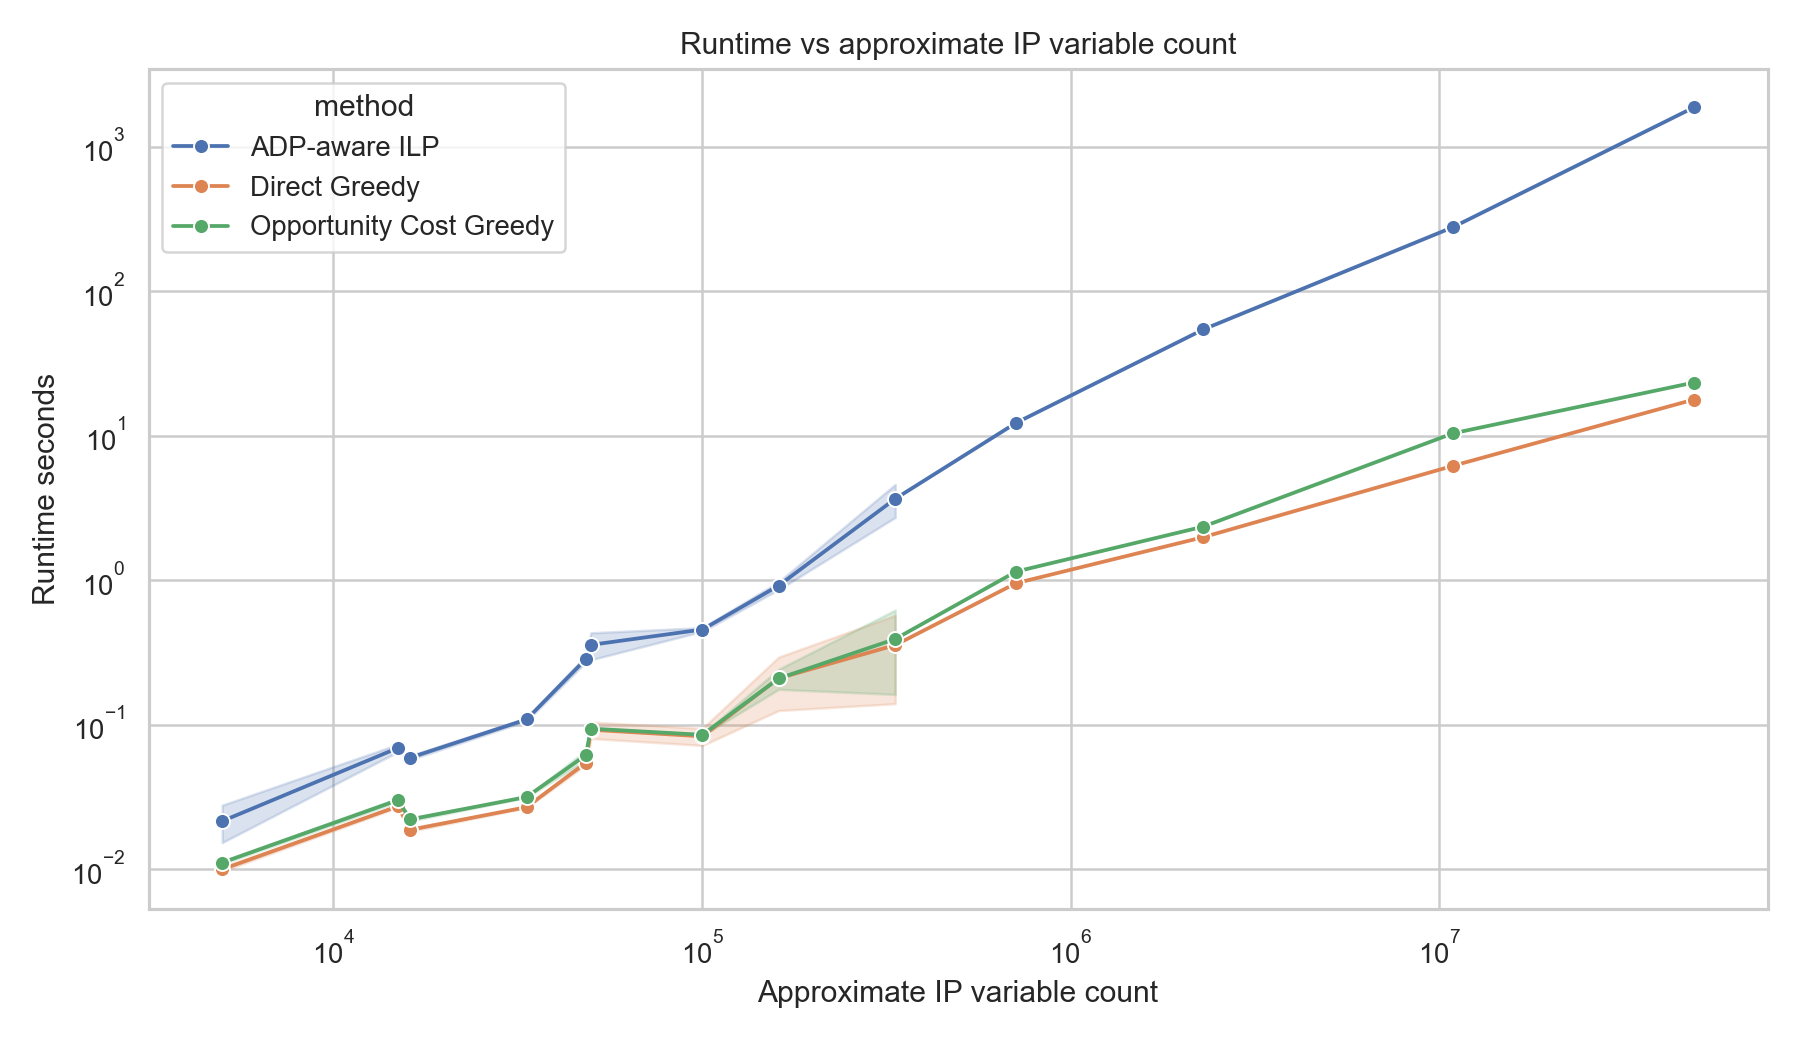
\includegraphics[width=0.88\linewidth]{experiments/synthetic/scaling_summary/runtime_by_variable_count.png}
  \caption{Runtime versus approximate IP variable count.}
\end{figure}

\begin{figure}[H]
  \centering
  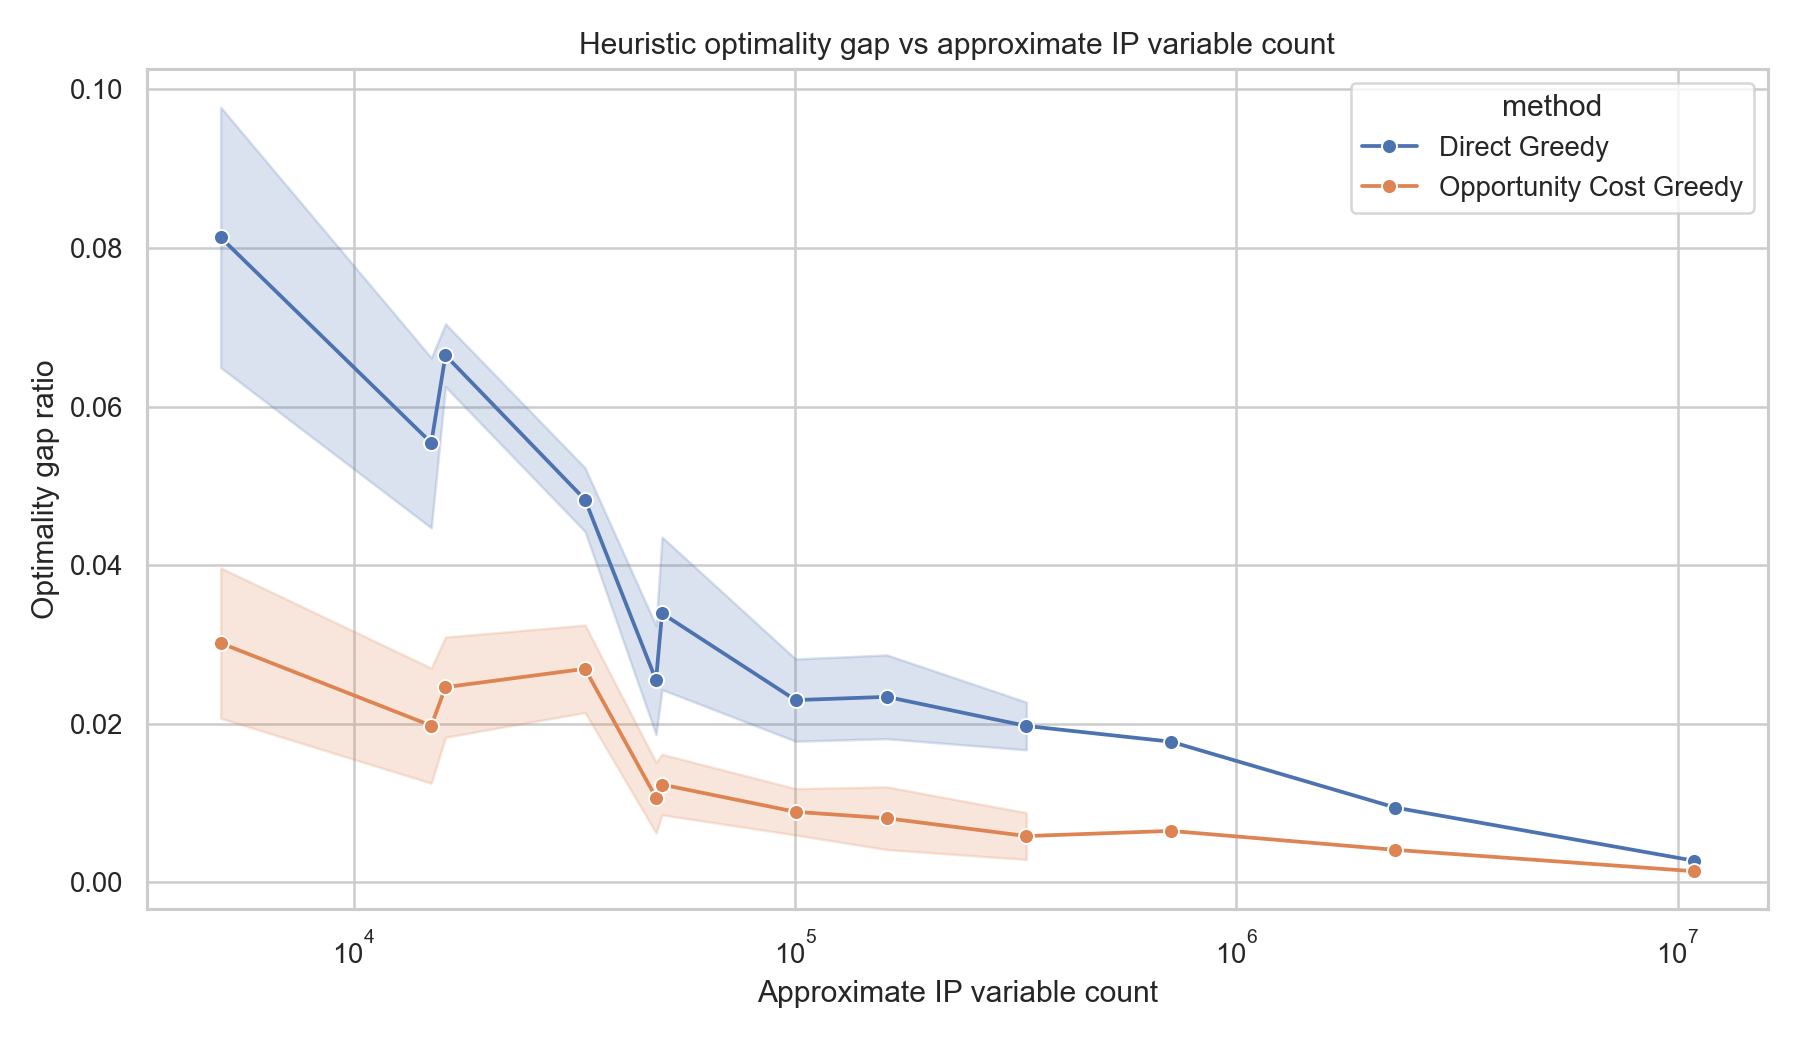
\includegraphics[width=0.88\linewidth]{experiments/synthetic/scaling_summary/heuristic_gap_by_variable_count.png}
  \caption{Heuristic optimal-gap percentage versus approximate IP variable count.}
\end{figure}

\begin{figure}[H]
  \centering
  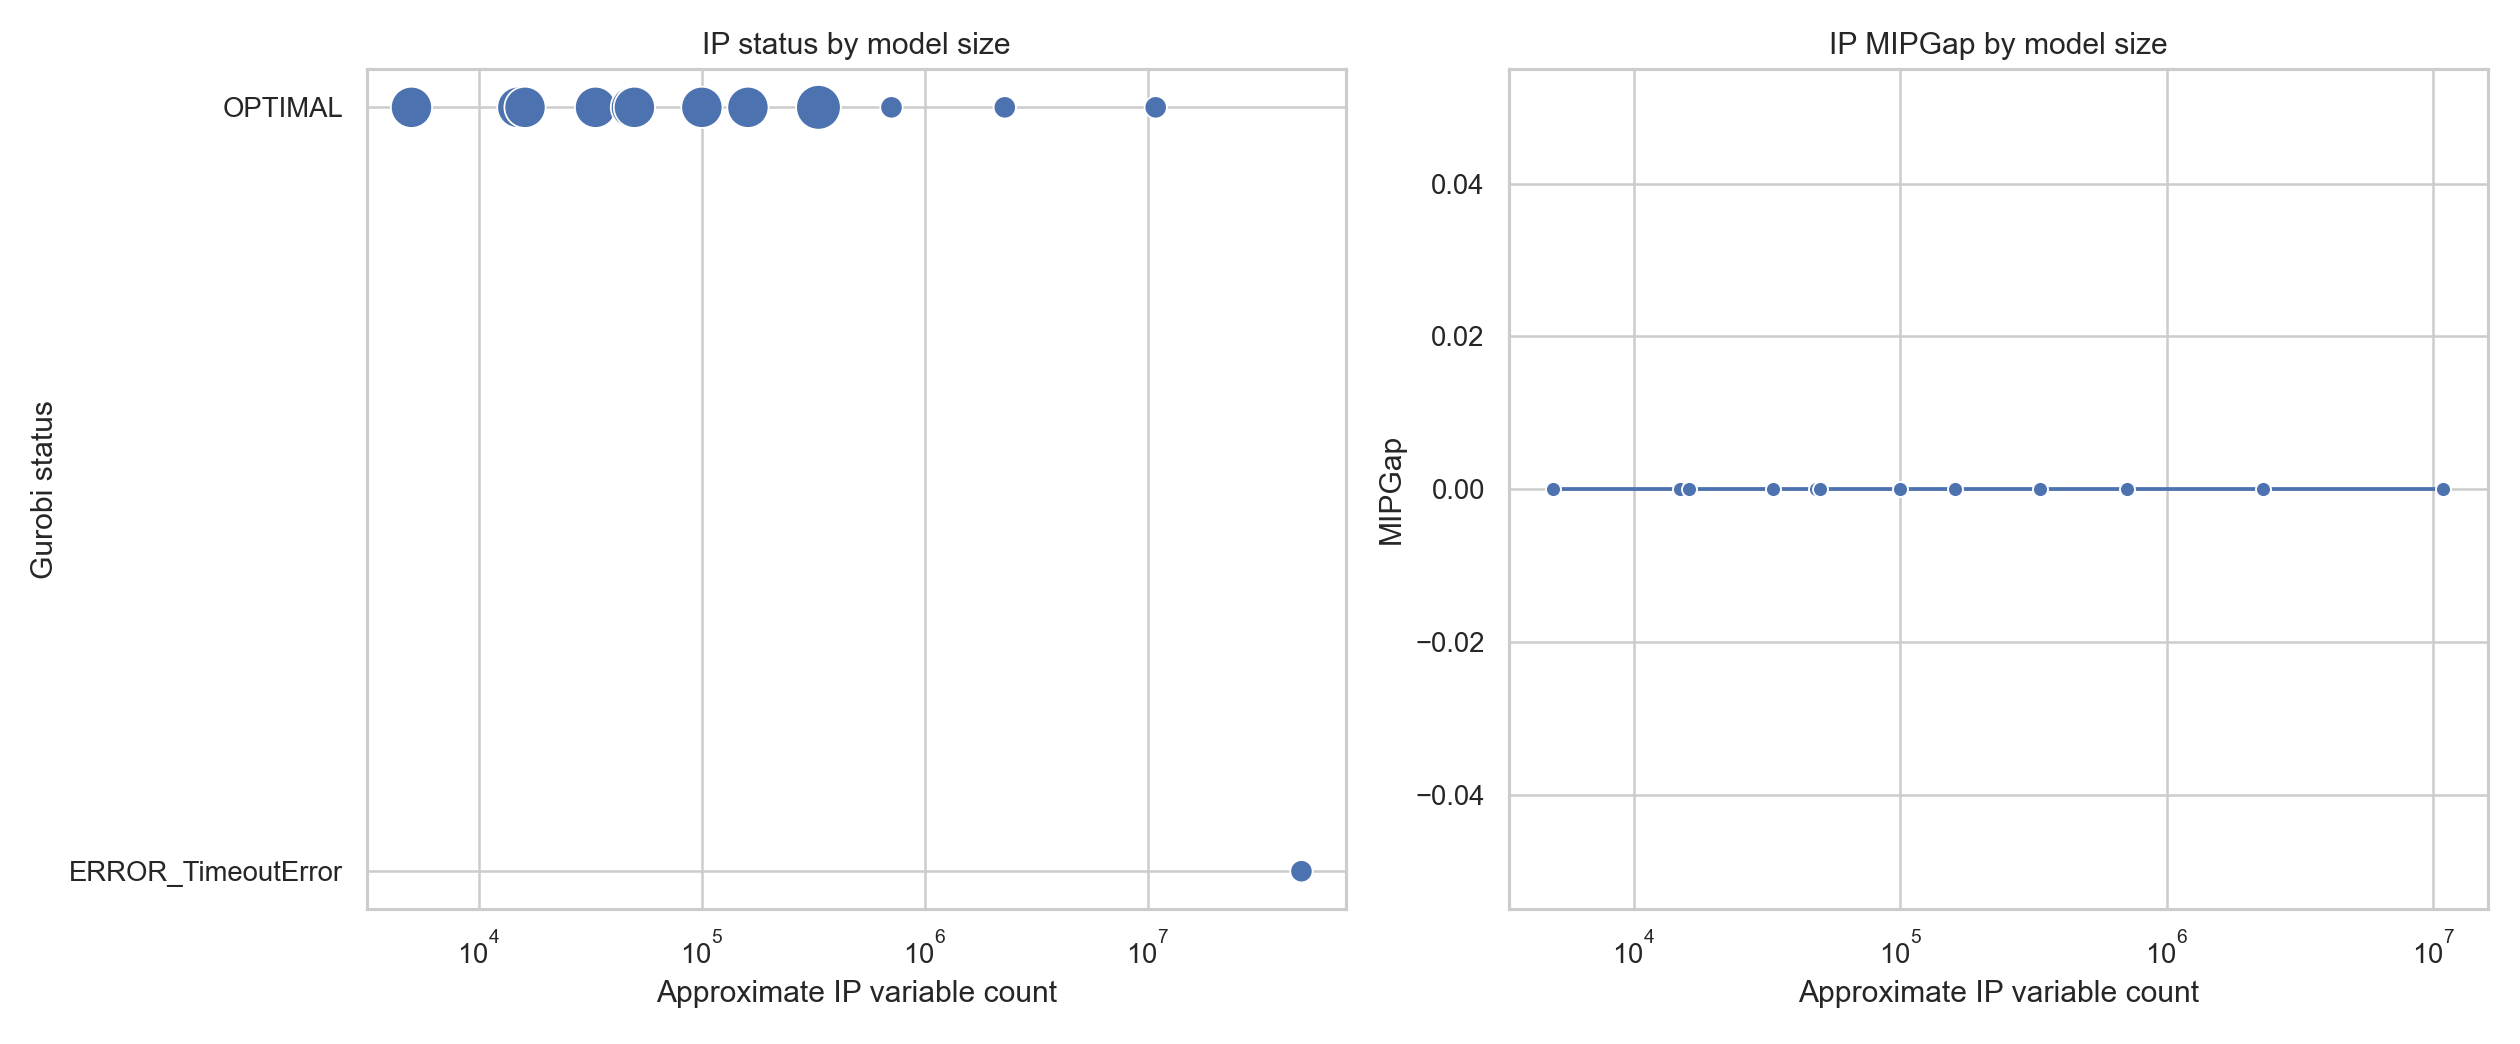
\includegraphics[width=0.88\linewidth]{experiments/synthetic/scaling_summary/ip_status_mip_gap_by_variable_count.png}
  \caption{ILP status and MIP gap versus approximate IP variable count.}
\end{figure}

\begin{table}[H]
\centering
\caption{Representative N6 stress-test results.}
\begin{tabular}{lrrrr}
\toprule
Instance & ILP time (s) & Direct Greedy (s) & OCG (s) & ILP status \\
\midrule
stress\_small & 4.235 & 0.790 & 0.852 & optimal \\
stress\_medium & 12.230 & 0.951 & 1.144 & optimal \\
stress\_large & 54.267 & 1.981 & 2.344 & optimal \\
stress\_xlarge & 276.895 & 6.172 & 10.360 & optimal \\
stress\_timeout\_target & 1869.805 & 17.760 & 23.286 & timeout \\
\bottomrule
\end{tabular}
\end{table}

\begin{table}[H]
\centering
\small
\setlength{\tabcolsep}{4pt}
\caption{N6 stress sizes used for runtime scaling.}
\label{tab:n6_size}
\begin{tabular}{lrrr}
\toprule
Instance & Approx. variables & Players & Roster size \\
\midrule
stress\_small & 334,080 & 5,760 & 48 \\
stress\_medium & 710,400 & 9,600 & 64 \\
stress\_large & 2,289,600 & 21,600 & 96 \\
stress\_xlarge & 10,880,000 & 64,000 & 160 \\
stress\_timeout\_target & 49,029,120 & 184,320 & 256 \\
\bottomrule
\end{tabular}
\end{table}

\subsection{Real-data validation}

The real-data validation uses 2026 Yahoo and FanGraphs player pools. Each dataset contains 252 draft cases. These cases are not the main scalability evidence, because they do not isolate factors the way the synthetic design does, but they show that the same method ranking appears on realistic fantasy-baseball inputs.

\begin{table}[H]
\centering
\small
\caption{Real-data validation summary. Optimal gap is measured in projected points.}
\label{tab:real_data}
\begin{tabular}{llrrr}
\toprule
Dataset & Method & Mean objective & Mean gap & Max gap \\
\midrule
Yahoo 2026 & ADP-aware ILP & 7917.209 & 0.000 & 0.000 \\
Yahoo 2026 & Opportunity Cost Greedy & 7767.732 & 149.477 & 255.700 \\
Yahoo 2026 & Direct Greedy & 7662.866 & 254.343 & 373.000 \\
\midrule
FanGraphs 2026 & ADP-aware ILP & 14642.927 & 0.000 & 0.000 \\
FanGraphs 2026 & Opportunity Cost Greedy & 14320.135 & 322.792 & 508.000 \\
FanGraphs 2026 & Direct Greedy & 14097.337 & 545.590 & 644.500 \\
\bottomrule
\end{tabular}
\end{table}

The real-data result is consistent with the synthetic story. On Yahoo, Opportunity Cost Greedy reduces the mean gap from 254.343 points to 149.477 points. On FanGraphs, it reduces the mean gap from 545.590 points to 322.792 points. The absolute point scales differ across the two projection systems, but the ranking of methods is the same.

\subsection{Factor-level lessons}

The point-distribution factor shows that the value landscape changes the cost of mistakes. The high-low setting creates a small elite group, so a draft rule that waits too long can lose value quickly. This is where Direct Greedy performs worst in N2. Opportunity Cost Greedy still loses some value relative to the ILP, but the gap is much smaller because the method explicitly prices the cost of delay.

The position-distribution factor shows that roster feasibility is not a secondary detail. Single-position players make early mistakes harder to repair, while flexible players give the algorithm more ways to satisfy the final roster. Opportunity Cost Greedy performs well in both cases because it checks the future availability of each open position instead of treating all roster needs as interchangeable.

The scaling factor separates quality from computational practicality. In N4, both roster scale and player-demand ratio change the structure of the problem. A larger roster increases the number of required decisions, while a larger player pool increases the number of alternatives the model must consider. The ILP can solve the moderate cases, but the N6 stress cases show why exact optimization is not the right operational tool at the largest scales.

The ADP factor captures market uncertainty. Low $\sigma_{\text{adp}}$ means ADP is reliable, so availability is easier to predict. Higher noise makes the market less predictable, and both heuristics become less accurate. Opportunity Cost Greedy remains better because it directly uses the next-pick availability comparison, which is the same business question a manager faces during a snake draft: whether a player or position will still be there next time.

Together, the factors show that the proposed heuristic is useful for more than one reason. It helps when points are concentrated among elite players, when positions are scarce, when ADP is noisy, and when exact optimization becomes slow. That combination is stronger evidence than a single aggregate score.

\subsection{Overall experimental interpretation}

Across N1--N5, Opportunity Cost Greedy consistently reduces the optimal gap relative to Direct Greedy. The improvement is visible in the baseline case, in elite-heavy point distributions, in constrained position structures, in scale experiments, and under ADP uncertainty. This matters because the heuristic is not tuned only for one synthetic setting; it remains useful across multiple draft environments.

N6 then adds the runtime argument. The ILP is still useful as a benchmark, but the stress results show where exact optimization becomes operationally expensive. At the largest stress target, the ILP exceeds the 1800-second wall-time target, while both heuristics still finish in seconds. Therefore, the practical recommendation is not to replace the ILP as a benchmark, but to use Opportunity Cost Greedy as the scalable draft-decision method.

Direct Greedy remains important because it represents a realistic simple rule. The fact that Opportunity Cost Greedy improves on it across the factor table shows that the opportunity-cost calculation contributes meaningful decision value rather than only extra computation.

\section{Conclusions}

This project treats fantasy baseball draft planning as an operations research decision problem. The core challenge is to build a feasible and high-value roster under positional constraints, market timing, and limited draft opportunities. To study that problem, we formulated an ADP-aware ILP benchmark and compared it with Direct Greedy and the self-designed Opportunity Cost Greedy heuristic.

The empirical message is straightforward. The ILP is the strongest benchmark but becomes expensive as instances scale. Direct Greedy is fast, but it is too myopic to fully account for the cost of waiting. Opportunity Cost Greedy offers the best balance for practical use because it keeps the strategic structure of the exact model while staying much more scalable.

The main limitation is that ADP is only a proxy for future availability. In real drafts, opponents do not follow ADP mechanically, so the market signal can be noisy. Projected points are also uncertain and can change over time, especially when injuries, role changes, or lineup decisions alter the expected value of a player. Finally, the current model focuses on the starting roster and does not explicitly model bench management or category-specific strategic behavior.

These limitations also suggest natural extensions. A richer future version of the project could include opponent behavior models, probabilistic projection intervals, bench-value logic, or a hybrid repair step that uses the heuristic to create a good initial solution and then applies limited exact optimization to improve it. Those directions would preserve the core insight of the current report while making the model closer to a full fantasy-management tool.

Overall, the report supports a practical recommendation: when a fantasy manager needs a fast but strategic draft tool, Opportunity Cost Greedy is a stronger choice than a simple greedy baseline, while the ILP remains useful as an exact benchmark for analysis and validation.

\end{document}
